\documentclass[a4paper,12pt]{article}
\usepackage[utf8]{inputenc}
\usepackage{hyperref}
\usepackage[T1]{fontenc}
\usepackage{typearea}
\usepackage{scrpage2}
\usepackage{vmargin}
\usepackage{color}
\usepackage{fancyvrb}
\usepackage{listings}
\usepackage{tocloft}
\usepackage{graphicx}
\lstset{inputencoding=ansinew}
\usepackage{spreadtab}
\usepackage{framed}
\hypersetup{pdfstartview=FitH}
\hypersetup{%
    pdfborder = {0 0 0}
}

\begin{document}
\thispagestyle{empty}
\begin{center}
 
\includegraphics[width=0.16\textwidth]{resources/informatik_logo}

\includegraphics[width=0.55\textwidth]{resources/tu_logo}\\[1cm]
\newcommand{\HRule}{\rule{\linewidth}{0.5mm}}
\HRule \\[0.4cm]
{ \Large \bfseries Einführung in paralleles Rechnen\\
Wintersemester 2015\\ [0.2cm]
Projekt 2: Merging \\ [0.2cm]
Bericht}\\[0.4cm]

\HRule \\[1.5cm]
{\large
Stefan Karner, 1027209 \hfill Enri Miho, 0929003
}
\end{center}

\newpage
\tableofcontents
\newpage
\section{Problemstellung}
	In diesem Bericht stellen wir einen parellelen Algorithmus vor, der 2 gegebene Arrays mit den Längen $m$ und $n$ in ein Array der Länge $m + n$ zusammenfügt. Beide Input-Arrays sind schon aufsteigend sortiert. Das resultierende Array muss dann auch aufsteigend sortiert sein. Dabei muss der Algorithmus für \emph{jede Array Größe} und \emph{jede Anzahl von Prozessoren/Threads} funktionieren.\\
Implementiert wird das ganze in der Programmierprache c. Der parallele Algorithmus wird mit der Hilfe von 3  Frameworks implementiert (jeweils eine Implementierung für jedes Framework):
\begin{itemize}
\item OpenMP: eine API für Shared-Memory-Programmierung
\item Cilk: eine Art Programmiersprache für parellele Berechnungen, die auf die Programmierprache c aufbaut
\item MPI: ein Interface, das den Austausch von Nachrichten  bei parallelen Berechnungen auf verteilten Systemen ermöglicht
\end{itemize}
Wichtig dabei ist, dass alle Prozessoren ungefähr gleich viel zu tun haben (workload balancing). Das heißt die Arrays die jeder Prozessor übergeben bekommt haben alle ungefähr die gleiche Länge. Wie das erreicht werden kann, wird später erklärt.\\
Anschließend müssen die Laufzeiten von jeder dieser parellelen Implementierungen mit der Laufzeit der sequentiellen Referenzimplementierung verglichen werden. Das Zeil ist zu analysieren wie viel schneller die parallelen Programme sind. Die Zahl die das angibt nennt man \emph{Speedup} und ist definiert durch:
\begin{center}
$ S = \frac{T_{seq}}{T_{par}}$
\end{center}
wobei $T_{seq}$ die Ausführungszeit der sequentiellen Implementierung ist und $T_{par}$ die der parallelen.

\section{Der Algorithmus}
	\subsection{Der sequentielle Algorithmus}
Der sequentielle Algorithmus vergleicht in jedem Durchlauf die Werte an den aktuellen Indizes beider Input-Arrays. Der Index wird erhöht für das Array das beim Vergleich den kleineren Wert (dieser wird in das resultierende Array geschrieben) hat. Erreicht man das Ende eines der beiden Arrays, werden die übrig gebliebenen Elemente des anderen in das resultierende Array geschrieben (ab dem aktuellen Index).

\subsection{Der parallele Algorithmus}
Der Übergang vom sequentiellen Algorithmus zum parallelen ist nicht trivial. Das Problem besteht darin, dass jeder Durchlauf von den vorigen abhängt. Die Idee ist die Input-Arrays so zu zerteilen, dass die Prozessoren dann mit diesen Teilen unabhängig von einander arbeiten können.

Es wurden zu Beginn einige Ansätze untersucht, die auch in den Folien beschrieben sind. Gewählt wurde am Ende der letzte, \emph{merging by co-ranking}, da bei diesem Ansatz alle Prozessoren Teile gleicher Länge übergeben kriegen. Außerdem überschreitet die Anzahl der Prozessoren $(m+n) / log min(m,n)$ nicht, das heißt der Speedup des Algorithmus ist \emph{optimal}. Der Algorithmus wurde mit Hilfe eines Papers~\cite{corank} konzipiert.

Bevor der Algorithmus erklärt wird, geben wir die Definition des \emph{co-ranks}. Sei $merge$ die Funktion, für die gilt:
\begin{center}
$C[0,\dots,i-1] = merge(A[0,\dots,j-1], B[0,\dots,k-1])$
\end{center}
Dann nennt man die Indizes $j$ und $k$ die \emph{co-ranks} von $i$.

\section{Implementierung}
	\subsection{OpenMP}
Wie man dem Code entnehmen kann, sind $start$ und $end$ die Grezen für jeden Durchlauf, also von wo bis wo jeder Prozess in das resultierende Array schreiben soll. Die Grenzen für die Input-Arrays (aus denen gelesen wird) werden durch die $coranks$-Implementierung die wir vorgestellt haben, bestimmt.\\
Mit Hilfe von den Konstrukten von OpenMP kann erreicht werden, dass jeder Durchlauf von einem eigenen Prozessor durchgeführt wird. 
\begin{verbatim}
#pragma omp parallel
{
    #pragma omp for
    for (int i=0; i<p; i++) {
        int startA, endA, startB, endB;
        long start = (long)i*(long)(lenA+lenB)/(long)p;
        long end = (long)(i+1)*(long)(lenA+lenB)/(long)p;
        coranks(start, A, lenA, &startA, B, lenB, &startB);
        coranks(end, A, lenA, &endA, B, lenB, &endB);
        sequential_merge(A+startA, endA-startA, B+startB, 
             endB-startB, result+start);
    }
}
\end{verbatim}
Die Durchläufe finden also parallel statt. Die Prozesse/Threads arbeiten dabei unabhängig von einander, kommen sich also nicht in die Quere. Da die Grenzen eindeutig bestimmt sind, können mehrere Prozesse gleichzeitig das resultierende Array mit den verschmelzten Daten befüllen, indem sie die sequentielle Implementierung aufrufen.

\subsection{Cilk}

\subsection{MPI}

\section{Testumgebung}
	Wir haben eine Testumgebung entwickelt, die es uns erlaubt automatisiert zu testen sowie Ausführungszeiten zu messen und anschließend zu plotten.
In diesem Abschnitt wird ihr grundlegender Aufbau näher erläutert.
Konkrete Details zu den unterschiedlichen Testszenarien sind in Abschnitt 5 zu finden.

Die Testumgebung besteht aus einer Reihe von C-Programmen und Shell Skripts, sowie einem \texttt{gnuplot} Skript, das für die grafische Darstellung der Benchmarks zuständig ist.
Für jede parallele Implementierung existiert ein C-Programm, das sich um die Ausführung der einzelnen Testfälle kümmert.
Als einzigen Parameter verlangt es die Anzahl der Worker, die für das parallele Mergen eingesetzt werden sollen.

Die Testprogramme führen nun für eine Reihe von Testfällen sowohl die sequentielle, als auch die jeweilige parallele Implementierung aus.
In MPI kümmert sich ausschließlich der \emph{Master}prozess (Prozess mit dem Rank 0) um die Ausführung der Tests.
Alle anderen Prozesse sind \emph{Slaves} und warten nach dem Start direkt auf die Verteilung der zu mergenden Arrays.
Um rauscharme Ergebnisse zu erhalten, wird jeder Testfall 100 mal ausgeführt.
In jeder Ausführung misst die Testumgebung mit, wie lange die jeweilige Implementierung für das Mergen der Daten gebraucht hat.
Anschließend werden die kleinsten und mittleren Ausführungszeiten der parallelen Implementierungen zusammen mit den erhaltenen Speedups (gruppiert nach Testfall und Implementierung) in Log-Dateien geschrieben.

Um die Korrektheit der implementierten Algorithmen zu gewährleisten wird bei jedem Testdurchlauf das Ergebnisse der sequentiellen Implementierung mit jenem der parallelen verglichen.
Kommt es hier zu einer Diskrepanz, wird der entsprechende Testfall in einem Error-Log festgehalten.
Da es während der Ausführung unserer Tests zu keinerlei Fehlern kam, gehen wir davon aus, dass die parallelen Implementierungen korrekt umgesetzt wurden.

Ferner existieren drei Shell Skripts, die die Ausführung der Tests auf den Rechnerclustern, sowie die Generierung der Plots automatisieren.
Das Skript \texttt{test.sh} lädt den Quellcode sowie je ein weiteres Shell Skript auf die beiden Cluster \emph{Saturn} und \emph{Jupiter} hoch.
Anschließend ruft es die beiden hochgeladenen Skripts auf, welche die Ausführung der Tests auf den jeweiligen Maschinen koordinieren.
Jedes der genannten Testprogramme wird nun von dem zuständigen Skript mit unterschiedlichen Anzahlen von Workern aufgerufen.
Im Abschluss lädt \texttt{test.sh} die erstellten Benchmarks herunter und stellt diese mit gnuplot grafisch dar.
	
\section{Testfälle}
	\input{chapters/Testfaelle}
	
\section{Ergebnisse}
	Allgemein ist zu sagen, dass es nicht einfach war einigermaßen plausible Ergebnisse zu erhalten.
Die Prozessorauslastung schwankte zumeist sehr stark, da viele Benutzer gleichzeitig auf den Maschinen testeten.
Aus diesem Grund kam es gelegentlich zu ungewöhnlich hohen Ausführungszeiten bei den parallelen Implementierungen, insbesondere bei Verwendung vieler Prozessoren.
Um dieses Problem abzuschwächen, ließen wir unsere Testsskripts mehrmals durchlaufen und warteten stets darauf, dass möglichst wenige Benutzer auf den Maschinen aktiv sind.

Wir haben zwei verschiedene Arten von Plots erstellt.
Zum einen wird die mittlere Ausführungszeit eines Tests als Funktion der Testgröße dargestellt.
Die Größe bezieht sich hierbei auf die Elemente eines einzelnen Arrays.
Das gemergte Array umfasst also doppelt so viele Elemente wie im Plot angegeben.
Zum anderen wird der erreichte Speedup als Funktion der Prozessorzahl visualisiert.

Der erreichte Speedup ist sehr stark von der Testgröße abhängig.
Sind die Arrays zu klein, ist der Synchronisations- bzw. Kommunikationsoverhead zu groß und es kann kein Nutzen aus der größeren Prozessorzahl gezogen werden.
Je mehr Prozesse resp. Threads beteiligt sind, desto größer wird der Overhead.
Bei einer sehr kleinen Arraygröße, wie 1000, kommt es daher bei allen parallelen Implementierungen zu einer deutlichen Verlangsamung im Vergleich zur sequentiellen Implementierung.
Erst ab einer Größe von etwa 100000 Elementen pro Array ist bei nahezu allen Implementierungen ein Geschwindigkeitsanstieg zu verzeichnen. 


\subsection{Cilk}
Mit Cilk konnten wir einen moderaten Speedup erzielen.
Aus den Abbildungen \ref{Cilk_Disjunct_sizes} und \ref{Cilk_Interleaved_sizes} ist ersichtlich, dass der Speedup bei ausreichend großen Testfällen anfangs schnell ansteigt, dann jedoch stagniert.
Wie zu erwarten, ist der Speedup bei komplett unabhängigen Arrays etwas größer als bei perfekt verzahnten.
Dennoch kamen wir selbst bei einer Testgröße von $n = 500000$ kaum über den Faktor 6 hinaus.
Eingedenk der Tatsache, dass der maximal mögliche Geschwindigkeitszuwachs bei 48 liegt, wirken die Ergebnisse der Cilk-Implementierung relativ bescheiden.
Eine grafische Übersicht der Benchmarks ist in den Abbildungen \ref{Cilk_Disjunct_sizes}, \ref{Cilk_Disjunct_cores}, \ref{Cilk_Interleaved_sizes} und \ref{Cilk_Interleaved_cores} zu finden.


\begin{figure}[p]
	\centering
	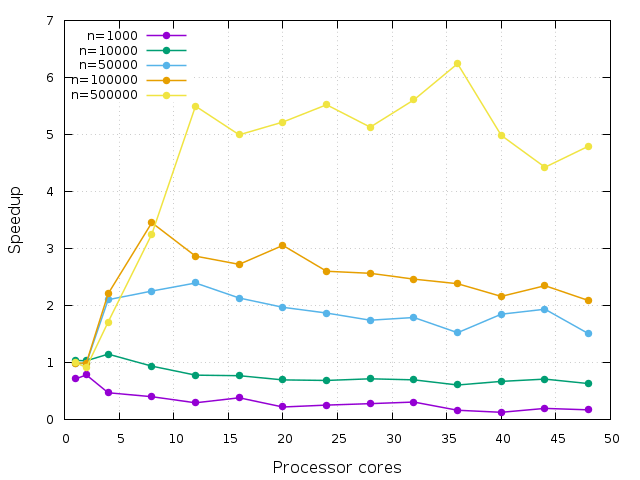
\includegraphics[width=404pt]{resources/plots/Cilk_Disjunct_sizes.png}
	\caption{Cilk (disjuct) - Speedup als Funktion der Prozessorkerne}
	\label{Cilk_Disjunct_sizes}
\end{figure}

\begin{figure}[p]
	\centering
	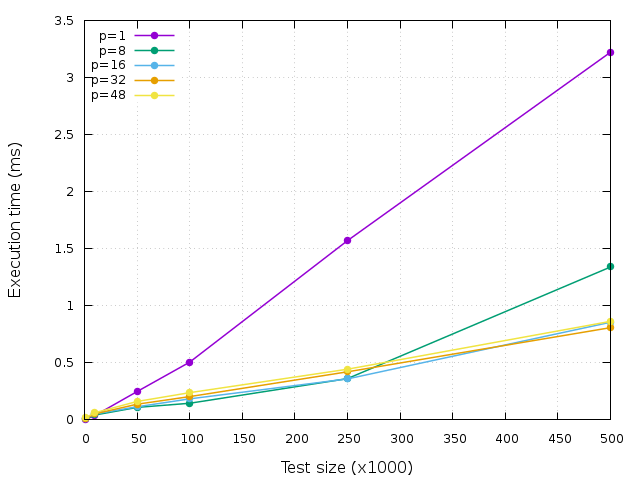
\includegraphics[width=404pt]{resources/plots/Cilk_Disjunct_cores.png}
	\caption{Cilk (disjuct) - Ausführungszeit als Funktion der Testgröße}
	\label{Cilk_Disjunct_cores}
\end{figure}

\begin{figure}[p]
	\centering
	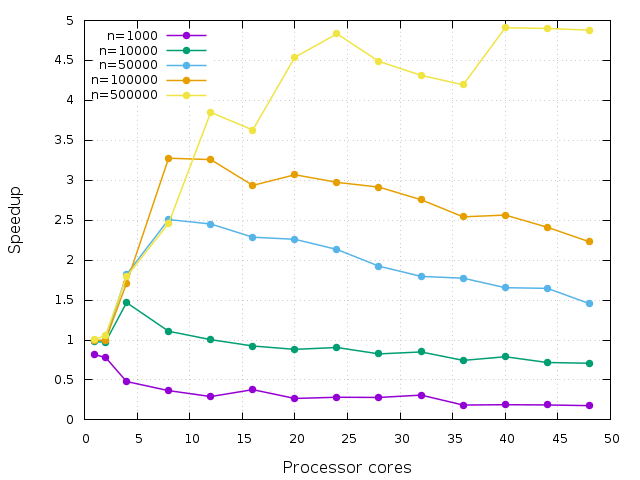
\includegraphics[width=404pt]{resources/plots/Cilk_Interleaved_sizes.png}
	\caption{Cilk (interleaved) - Speedup als Funktion der Prozessorkerne}
	\label{Cilk_Interleaved_sizes}
\end{figure}

\begin{figure}[p]
	\centering
	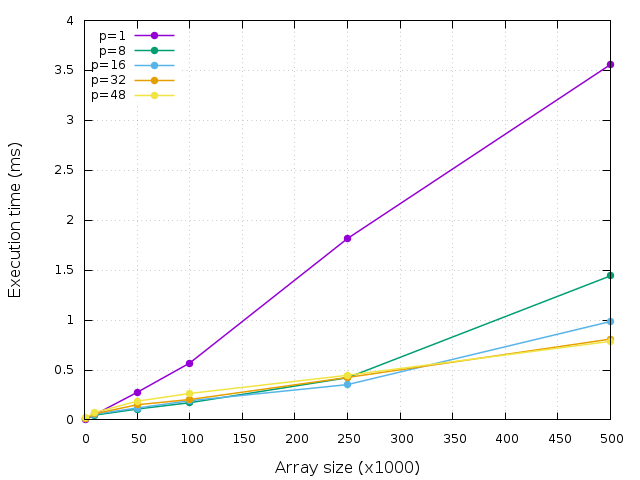
\includegraphics[width=404pt]{resources/plots/Cilk_Interleaved_cores.png}
	\caption{Cilk (interleaved) - Ausführungszeit als Funktion der Testgröße}
	\label{Cilk_Interleaved_cores}
\end{figure}



\subsection{OpenMP}
Im Gegensatz zu Cilk lieferte unsere Implementierung in OpenMP einen erstaunlich großen Speedup.
Sieht man sich die Abbildungen \ref{OpenMP_Disjunct_sizes} und \ref{OpenMP_Interleaved_sizes} an, kann man erkennen, dass der Speedup bei $n = 500000$ einigermaßen linear mit der Anzahl der Threads ansteigt.
In einigen Tests konnte sogar ein superlinearer Speedup erreicht werden.
Natürlich ist so ein Ergebnis in der Theorie nicht möglich.
Eine mögliche Erklärung hierfür ist, dass die Ausführung der sequentiellen Implementierung ungewöhnlich lange gedauert hat, weil die Prozessoren in dieser Zeit gut ausgelastet waren.
Nichtsdestotrotz scheint OpenMP für das gegebene Problem sehr gut geeignet zu sein.
Siehe auch die Abbildungen \ref{OpenMP_Disjunct_sizes}, \ref{OpenMP_Disjunct_cores}, \ref{OpenMP_Interleaved_sizes} und \ref{OpenMP_Interleaved_cores}.

Noch deutlicher als in Cilk sieht man den Unterschied zwischen den beiden Szenarien \emph{Interleaved} und \emph{Disjunct}.
Während der Speedup bei \emph{Disjunct} und $n = 500000$ den Faktor 50 deutlich übersteigt, ist bei \emph{Interleaved} bereits bei etwa 25 Schluss.


\begin{figure}[p]
	\centering
	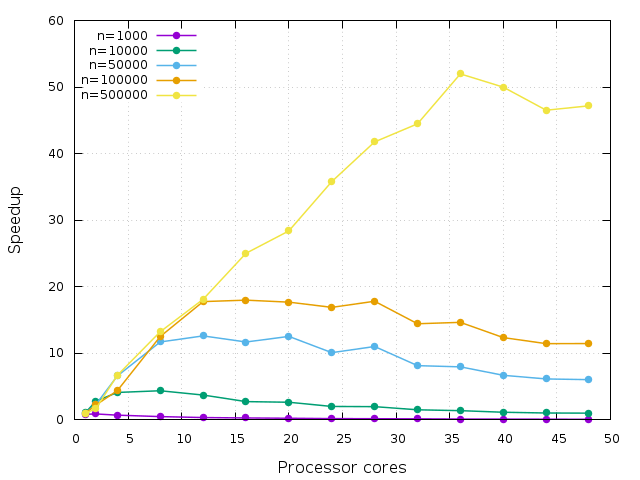
\includegraphics[width=404pt]{resources/plots/OpenMP_Disjunct_sizes.png}
	\caption{OpenMP (disjuct) - Speedup als Funktion der Prozessorkerne}
	\label{OpenMP_Disjunct_sizes}
\end{figure}

\begin{figure}[p]
	\centering
	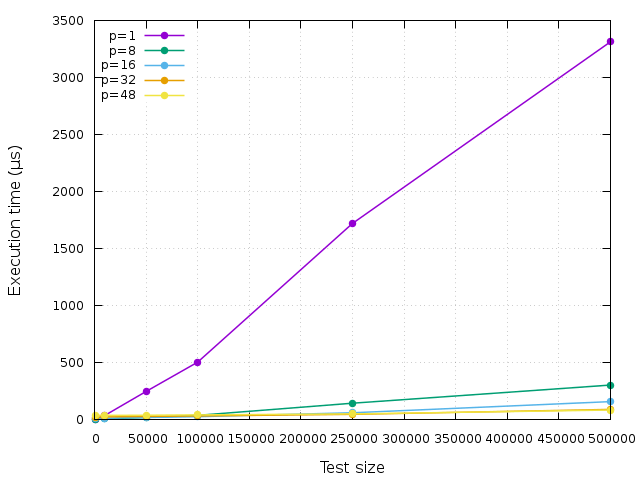
\includegraphics[width=404pt]{resources/plots/OpenMP_Disjunct_cores.png}
	\caption{OpenMP (disjuct) - Ausführungszeit als Funktion der Testgröße}
	\label{OpenMP_Disjunct_cores}
\end{figure}

\begin{figure}[p]
	\centering
	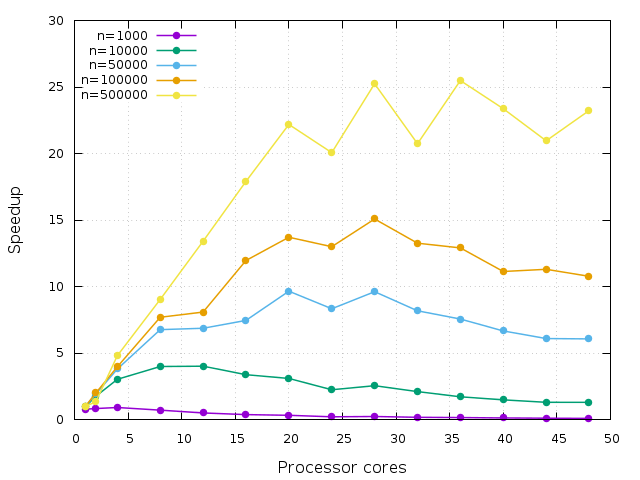
\includegraphics[width=404pt]{resources/plots/OpenMP_Interleaved_sizes.png}
	\caption{OpenMP (interleaved) - Speedup als Funktion der Prozessorkerne}
	\label{OpenMP_Interleaved_sizes}
\end{figure}

\begin{figure}[p]
	\centering
	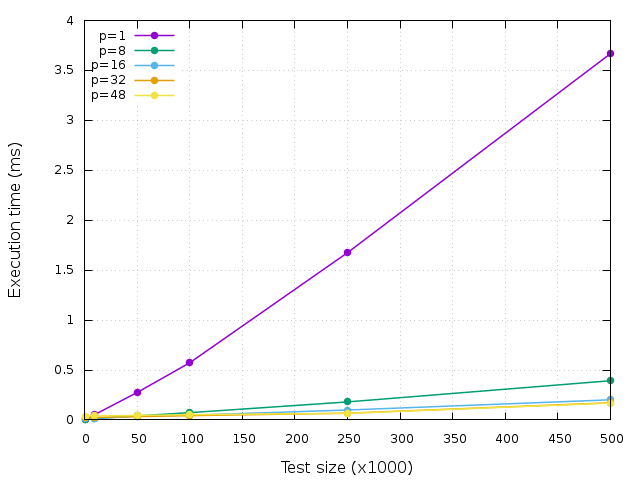
\includegraphics[width=404pt]{resources/plots/OpenMP_Interleaved_cores.png}
	\caption{OpenMP (interleaved) - Ausführungszeit als Funktion der Testgröße}
	\label{OpenMP_Interleaved_cores}
\end{figure}



\subsection{MPI}
Die Benchmarks der MPI-Implementierung haben uns sehr überrascht.
Selbst bei großen Arrays und vielen Prozessoren war nur ein sehr geringer Geschwindigkeitszuwachs zu verzeichnen.
In keinem der getesteten Szenarien kam der Speedup je über den Faktor 3 hinaus.
Spätestens ab einer Prozessorzahl von 100 kam es zudem zu keinem nennenswerten Anstieg der Geschwindigkeit mehr.
Es macht daher praktisch keinen Unterschied, ob 100 oder 500 Kerne zur Lösung des Problems verwendet werden.
Vergleiche hierzu die Abbildungen \ref{MPI_Disjunct_sizes}, \ref{MPI_Disjunct_cores}, \ref{MPI_Interleaved_sizes} und \ref{MPI_Interleaved_cores}.
Wir gehen davon aus, dass der Kommunikationsoverhead bei dem implementierten Algorithmus zu groß ist.


\begin{figure}[p]
	\centering
	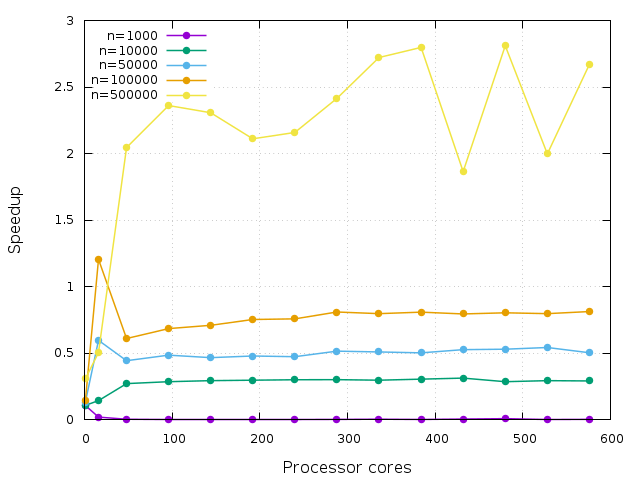
\includegraphics[width=404pt]{resources/plots/MPI_Disjunct_sizes.png}
	\caption{MPI (disjuct) - Speedup als Funktion der Prozessorkerne}
	\label{MPI_Disjunct_sizes}
\end{figure}

\begin{figure}[p]
	\centering
	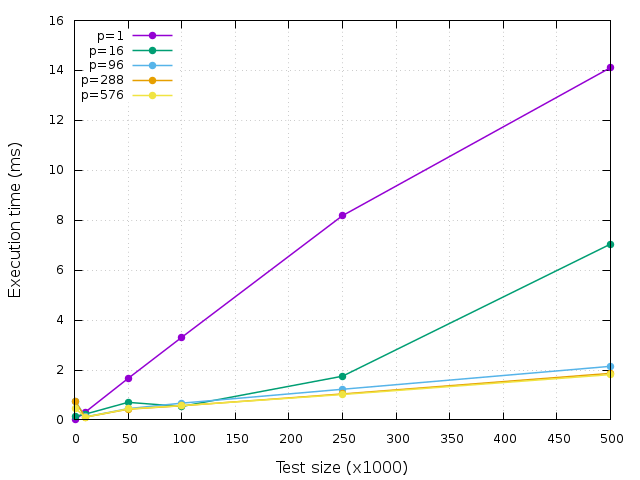
\includegraphics[width=404pt]{resources/plots/MPI_Disjunct_cores.png}
	\caption{MPI (disjuct) - Ausführungszeit als Funktion der Testgröße}
	\label{MPI_Disjunct_cores}
\end{figure}

\begin{figure}[p]
	\centering
	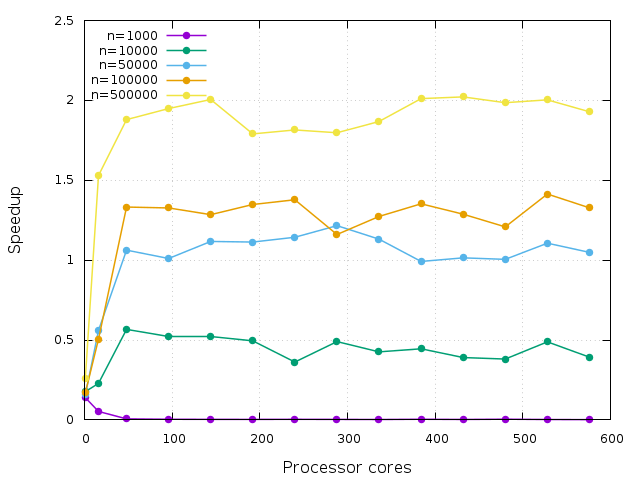
\includegraphics[width=404pt]{resources/plots/MPI_Interleaved_sizes.png}
	\caption{MPI (interleaved) - Speedup als Funktion der Prozessorkerne}
	\label{MPI_Interleaved_sizes}
\end{figure}

\begin{figure}[p]
	\centering
	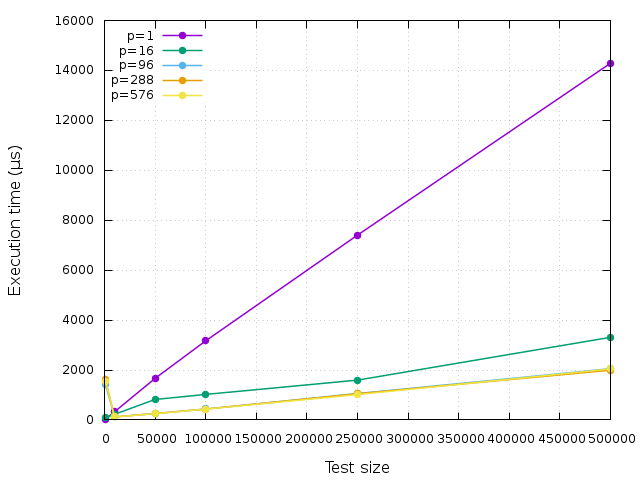
\includegraphics[width=404pt]{resources/plots/MPI_Interleaved_cores.png}
	\caption{MPI (interleaved) - Ausführungszeit als Funktion der Testgröße}
	\label{MPI_Interleaved_cores}
\end{figure}

	
\section{Fazit}
	\input{chapters/Fazit}

\newpage
\bibliographystyle{plain}
\bibliography{references}
\end{document}